\documentclass{article}
\usepackage{pgfplots}
\pgfplotsset{compat=1.18}

\begin{document}

\begin{figure}[h]
    \centering
    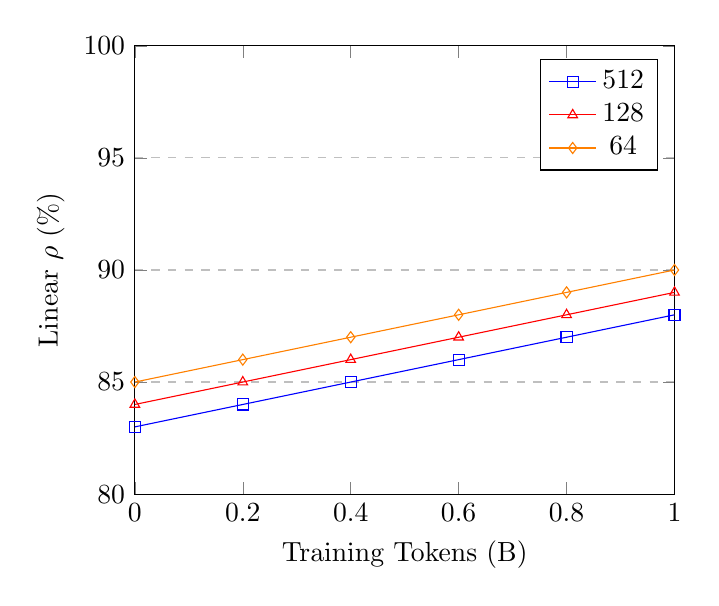
\begin{tikzpicture}
        \begin{axis}[
            xlabel={Training Tokens (B)},
            ylabel={Linear $\rho$ (\%)},
            xmin=0, xmax=1,
            ymin=80, ymax=100,
            xtick={0, 0.2, 0.4, 0.6, 0.8, 1},
            ytick={80, 85, 90, 95, 100},
            legend pos=north east,
            ymajorgrids=true,
            grid style=dashed,
        ]
            \addplot[
                color=blue,
                mark=square,
                ]
                coordinates {
                    (0, 83) (0.2, 84) (0.4, 85) (0.6, 86) (0.8, 87) (1, 88)
                };
            \addplot[
                color=red,
                mark=triangle,
                ]
                coordinates {
                    (0, 84) (0.2, 85) (0.4, 86) (0.6, 87) (0.8, 88) (1, 89)
                };
            \addplot[
                color=orange,
                mark=diamond,
                ]
                coordinates {
                    (0, 85) (0.2, 86) (0.4, 87) (0.6, 88) (0.8, 89) (1, 90)
                };
            \legend{512, 128, 64}
        \end{axis}
    \end{tikzpicture}
    \hfill
    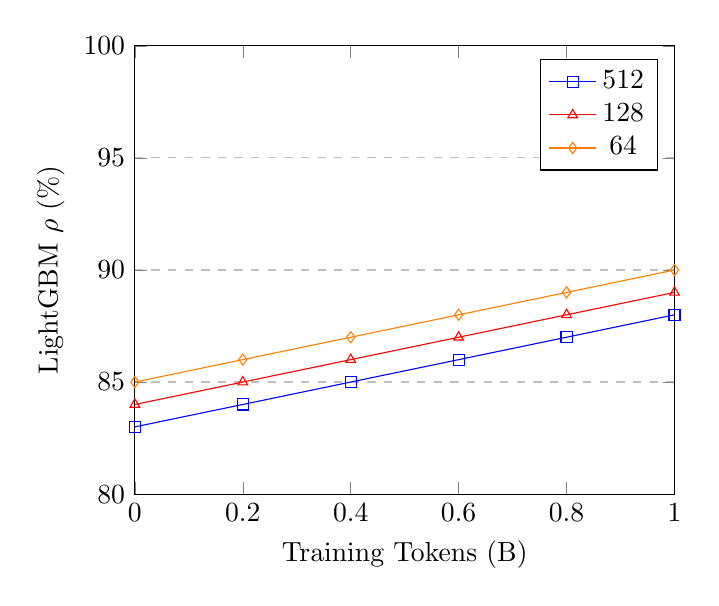
\begin{tikzpicture}
        \begin{axis}[
            xlabel={Training Tokens (B)},
            ylabel={LightGBM $\rho$ (\%)},
            xmin=0, xmax=1,
            ymin=80, ymax=100,
            xtick={0, 0.2, 0.4, 0.6, 0.8, 1},
            ytick={80, 85, 90, 95, 100},
            legend pos=north east,
            ymajorgrids=true,
            grid style=dashed,
        ]
            \addplot[
                color=blue,
                mark=square,
                ]
                coordinates {
                    (0, 83) (0.2, 84) (0.4, 85) (0.6, 86) (0.8, 87) (1, 88)
                };
            \addplot[
                color=red,
                mark=triangle,
                ]
                coordinates {
                    (0, 84) (0.2, 85) (0.4, 86) (0.6, 87) (0.8, 88) (1, 89)
                };
            \addplot[
                color=orange,
                mark=diamond,
                ]
                coordinates {
                    (0, 85) (0.2, 86) (0.4, 87) (0.6, 88) (0.8, 89) (1, 90)
                };
            \legend{512, 128, 64}
        \end{axis}
    \end{tikzpicture}
    \caption{The plot of Spearman Rank Correlation $\rho$ between the predicted ranks and true ranks of Linear regression (\textbf{Left}) and LightGBM regression (\textbf{Right}) across different training tokens and different number of proxy models. As shown, increasing the number of proxy models significantly boosts $\rho$, while adding more training tokens has diminishing returns.}
\end{figure}

\end{document}